\chapter{Experiments}

\section{Privacy Setups}
In meinen Experimenten werde ich jeweils fünf Privacy Setups anwenden um mein Vorgehen zu evaluieren. Das erste, \texttt{no-dp}, ist reines Federated Learning ohne Differential Privacy. 

Zwei weitere, \texttt{relaxed} und \texttt{strict}, sind Szenarios, in denen klassische Differential Privacy angewendet wird. Es findet keine Individualisierung statt. \texttt{relaxed} legt das am wenigsten strengste Privacy Budget an alle Clients an, \texttt{strict} das strengste.

Die letzten beiden Setups wenden individualisierte Privacy Budgets an. Dabei sind die Verteilungen der Budgets unter den Clients so gewählt, dass bei \texttt{individual-relaxed} häufiger die weniger strengen Budgets gezogen werden, als bei \texttt{individual-strict}. Die Verteilungen sind so gewählt wie bei \textcite[p. 8]{boenisch:2023}.

Die einzelnen Budgets der Setups passe ich jedoch an die Datensätze an, da ansonsten die Modelle teilweise nicht konvergieren.

\section{Datasets}

In dieser Arbeit wird der vorgeschlagene Algorithmus empirisch auf synthetischen und realistischen Datensätzen evaluieren. Dabei orientiere ich mich an \textcite{aldaghri:2023}. In ihrer Arbeit haben sie realistische Datensätze von Tensorflow Federated genutzt, nämlich MNIST und EMNIST. Darüber hinaus haben sie synthetische Datensätze basierend auf MNIST erstellt. In diesen haben sie die Bilder nach Ziffern gruppiert und die Daten für die einzelnen Clients jeweils aus einer dieser Gruppen gesamplet. Darüber hinaus wurden einzelne Ziffern nur privaten Clients zugewiesen und die Auswirkungen dieser Setups ausgewertet.

Wie \textcite{boenisch:2023} lege ich Gruppen von Clients mit unterschiedlichen Privacy Budgets $\epsilon$ zugrunde. Dabei wähle ich die Budgets und Gruppengrößen wie sie: $\epsilon_p = \{1,2,3\}$ und $(34\%, 43\%, 23\%)$ bzw. $(54\%, 37\%, 9\%)$. Darüber hinaus evaluiere ich das Training mit dem strengsten Budget für alle Clients und mit dem FedAvg ohne Privacy Garantien, um sinnvolle Baselines für meinen Algorithmus zu erhalten.

\subsection{Data Distribution Skews}

Ich habe mich dafür entschieden MNIST, SVHN und CIFAR-100 zu nutzen, da sie in meinen Augen einen großen Teil von realistischen Problemen bei der Verteilung der Daten im Federated Learning abdecken. Von \textcite[p. 18f]{kairouz:2021} werden folgende mögliche Probleme bezüglich der Verteilung der Datensätze benannt:

\subsubsection{Intra-Client Distribution Skew}
Die Daten der einzelnen Clients können Abhängigkeiten aufweisen, beispielsweise wenn sie in einer zeitlichen Abfolge sortiert vorliegen. Derartige Abhängigkeiten können aber durch das shufflen der einzelnen Datenpunkte gelöst werden.

\subsubsection{Feature Distribution Skew}
Die Verteilung der Features kann sich zwischen den Clients unterscheiden, auch wenn die die Wahrscheinlichkeit der Labels gegeben der Features, $P(y|x)$, die gleiche ist. Dies ist zum Beispiel bei MNIST zu beobachten, bei denen die einzelnen handschriftlichen Ziffern von Client zu Client unterschiedlich aussehen, siehe \autoref{fig:mnist-digits}.

\subsubsection{Label Distribution Skew}
Die Verteilung der Labels auf den Clients kann sich unterscheiden, beispielsweise aufgrund von regionalen Unterschieden. Beispielsweise können Kangaroos fast nur in Australien beobachtet werden. Diese Besonderheit ist im CIFAR-100 Datensatz zu sehen, bei dem die Schnittmenger der Labels zwischen Clients sehr viel geringer ist, als bei den anderen Datensätzen, siehe \autoref{fig:cifar-client-label-dist}.

\subsubsection{Other Distribution Skews}
Darüber hinaus werden weitere Verzerrungen erwähnt. Es kann sein, dass die bedingten Wahrscheinlichkeiten von Features und Labels sich unterscheiden, beispielsweise sieht ein Haus in den USA anders aus als in Europa, in beiden Fällen ist es aber ein Haus (\textit{concept drift}). Andersherum kann es auch sein, dass die gleichen Features anders gelabelt sind, beispielsweise weil manche Daten auch für Menschen ununterscheidbar sind.

Darüber hinaus kann es sehr unterschiedliche Mengen von Trainingsdaten geben. Dies ist ebenfalls bei dem MNIST Datensatz der Fall, bei dem die Standardabweichung der Anzahl der Beispiele sehr hoch ist, siehe \autoref{tab:dataset-statistics}.


\begin{figure}[tb]
	\centering
	\begin{subfigure}{0.3\textwidth}
		\centering
		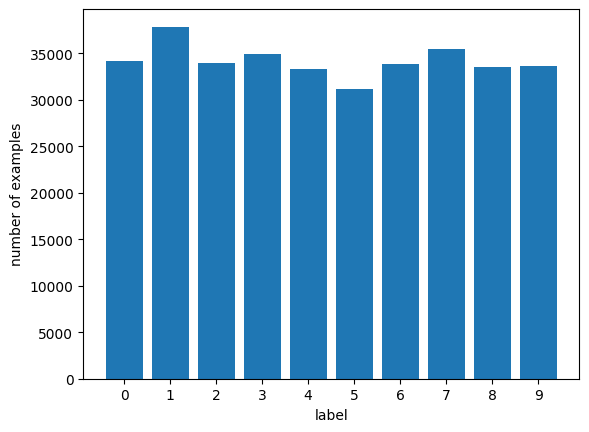
\includegraphics[width=\textwidth]{Bilder/emnist_label_distribution.png}
		\caption{EMNIST}
	\end{subfigure}
	\begin{subfigure}{0.3\textwidth}
		\centering
		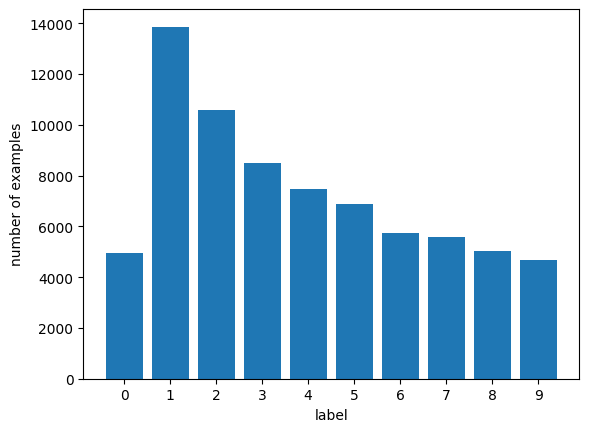
\includegraphics[width=\textwidth]{Bilder/svhn_label_distribution.png}
		\caption{SVHN}
	\end{subfigure}
	\begin{subfigure}{0.3\textwidth}
		\centering
		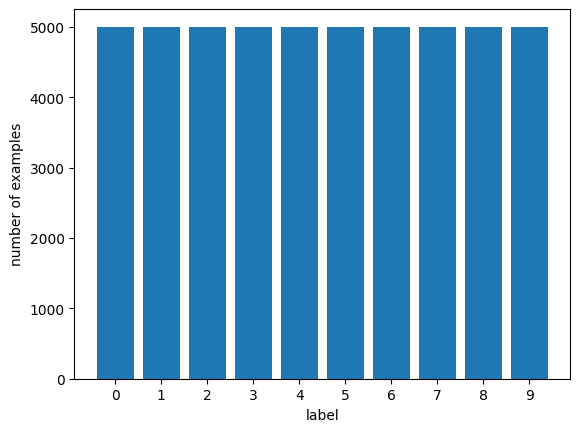
\includegraphics[width=\textwidth]{Bilder/cifar_label_distribution.png}
		\caption{CIFAR-100}
	\end{subfigure}
	\caption{Distribution of labels in the datasets among all clients}
\end{figure}

\begin{table}[tb]
	\centering
	\begin{tabular}{|c|c|c|c|c|c|c|c|}
		\hline
		\multirow{2}{4em}{Dataset} & \multicolumn{3}{|c|}{Whole Dataset} & \multicolumn{4}{|c|}{Per Client} \\
		\cline{2-8}
		& \#examples & \#classes & \#clients & $\diameter$examples & $\sigma$examples & $\diameter$classes & $\sigma$classes \\
		\hline
		MNIST & 341873 & 10 & 3383 & 101.05 & 14.72 & 9.99 & 0.14 \\
		SVHN & 26032 & 10 & 725 & 35.91 & 5.89 & 9.45 & 0.76 \\
		CIFAR-100 & 50000 & 20 & 500 & 100.0 & 0.0 & 6.53 & 1.99 \\
		\hline
	\end{tabular}
	\caption{Some statistics of the different datasets for (1) the whole dataset and (2) the individual clients}
	\label{tab:dataset-statistics}
\end{table}

\subsection{MNIST}
MNIST ist ein Datensatz, dessen Aufgabe eine Bildklassifizierung ist. Er besteht aus Graustufenbildern von handgeschriebenen Ziffern unterschiedlicher Autoren. Ziel ist es, die Bilder entsprechend der gezeigten Ziffer zu klassifizieren. Darüber hinaus gibt es EMNIST (Extended MNIST), der darüber hinaus auch Bilder von handgeschriebenen Buchstaben enthält \parencite{cohen:2017}. Dieser Datensatz ist in Tensorflow Federated integriert und wurde nach der Methode von \textcite{caldas:2018} aufeinzelne Clients aufgeteilt. Dabei werden jedem Client die Ziffern und Buchstaben eines Autors zugewiesen. \autoref{fig:mnist-digits} zeigt Beispiele für die Unterschiede der verschiedenen Handschriften. Dadurch kann der Datensatz die Heterogenität der Daten von unterschiedlichen Clients, die im Federated Learning auftritt, gut abbilden.

In meinem Experiment beschränke ich mich der Vergleichbarkeit halber nur auf die Ziffern aus dem Datensatz.

\begin{figure}[tb]
    \centering
    \begin{subfigure}{0.4\textwidth}
		\centering        
        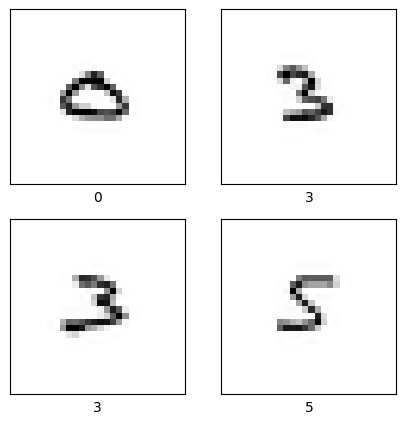
\includegraphics[width=\linewidth]{Bilder/emnist_client1.png}
        \caption{Client \texttt{f0599\_04} has 105 images in total}
    \end{subfigure}
    \hfill
    \begin{subfigure}{0.4\textwidth}
    		\centering        
        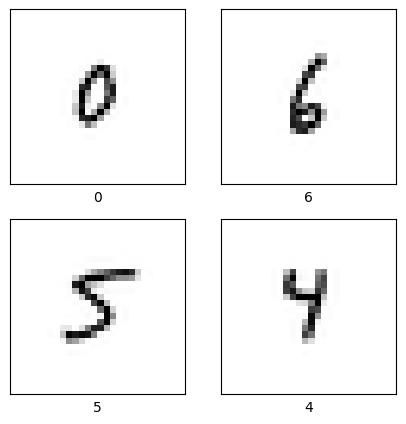
\includegraphics[width=\linewidth]{Bilder/emnist_client2.png}
        \caption{Client \texttt{f0654\_02} has 105 images in total}
    \end{subfigure}
    	\caption{Handwritten digits of different clients showing the difference in data distribution}
    \label{fig:mnist-digits}
\end{figure}

\begin{figure}[tb]
	\centering
	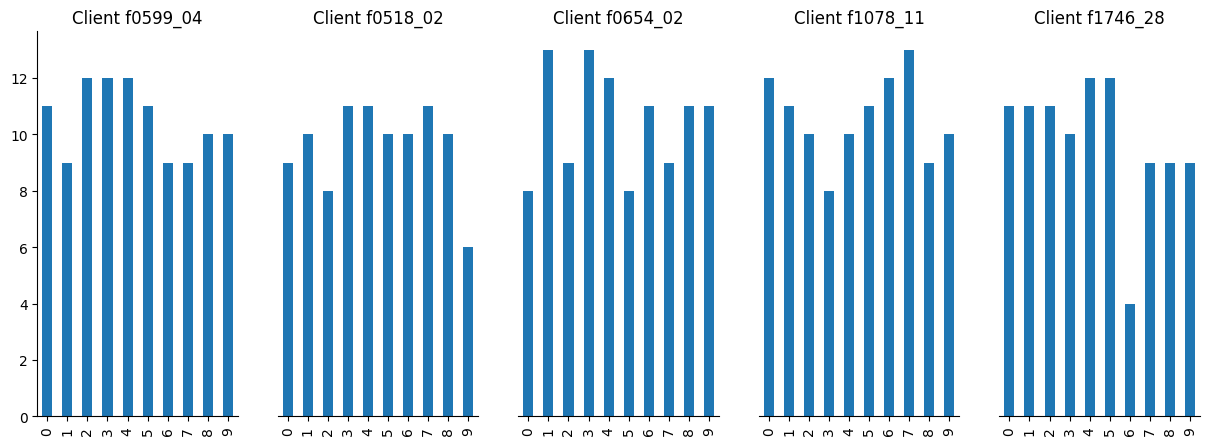
\includegraphics[width=\textwidth]{Bilder/emnist_client_label_distribution.png}
	\caption{}
	\label{fig:emnist-client-label-dist}
\end{figure}

\subsection{SVHN}

Der Street View House Numbers Datensatz \parencite{netzer:2011} ist ähnlich wie MNIST ein Datensatz um Ziffern zu erkennen. Allerdings liegen sie in diesem Fall als Bilder von Hausnummern aus Google Street View vor. Von dem Datensatz gibt es zwei Versionen: die erste enthält ganze Bilder und Bounding Boxes für jede Ziffer, die zweite enthält bereits gecroppte 32x32 Pixel große Bilder mit einzelnen Ziffern.

Für meine Arbeit habe ich die zweite Version genutzt. Um sie in Tensorflow Federated zu integrieren, habe ich die originalen Bilder im Matlab-Format eingelesen und sie auf eine feste Anzahl an Clients aufgeteilt. Eine Besonderheit ist, dass in dem Originaldatensatz die Zahl $10$ für eine $0$ steht. In meiner Version habe ich daher das Label $10$ durch $0$ ersetzt.

Um den Datensatz gut nutzen zu können, habe ich ihn in das \textit{SqlClientData}-Format\footnote{\url{https://www.tensorflow.org/federated/api_docs/python/tff/simulation/datasets/SqlClientData} (accessed: 2024-06-20)} von Tensorflow Federated gebracht und abgespeichert.

\begin{figure}[tb]
    \centering
    \begin{subfigure}{0.4\textwidth}
		\centering        
        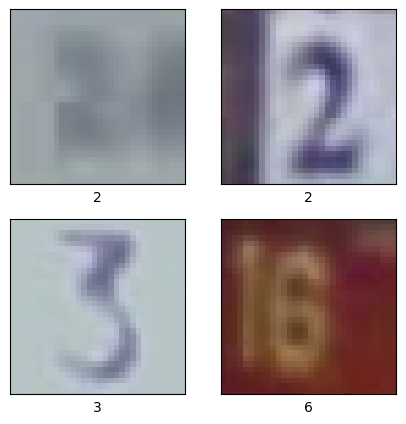
\includegraphics[width=\linewidth]{Bilder/svhn_client1.png}
        \caption{Client \texttt{client\_649} has 28 images in total}
    \end{subfigure}
    \hfill
    \begin{subfigure}{0.4\textwidth}
    		\centering        
        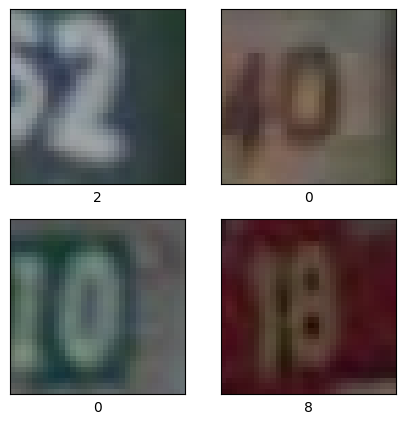
\includegraphics[width=\linewidth]{Bilder/svhn_client2.png}
        \caption{Client \texttt{client\_602} has 39 images in total}
    \end{subfigure}
    	\caption{Housenumbers of different clients. The individual digits were distributed randomly}
    \label{fig:svhn-digits}
\end{figure}

\begin{figure}[tb]
	\centering
	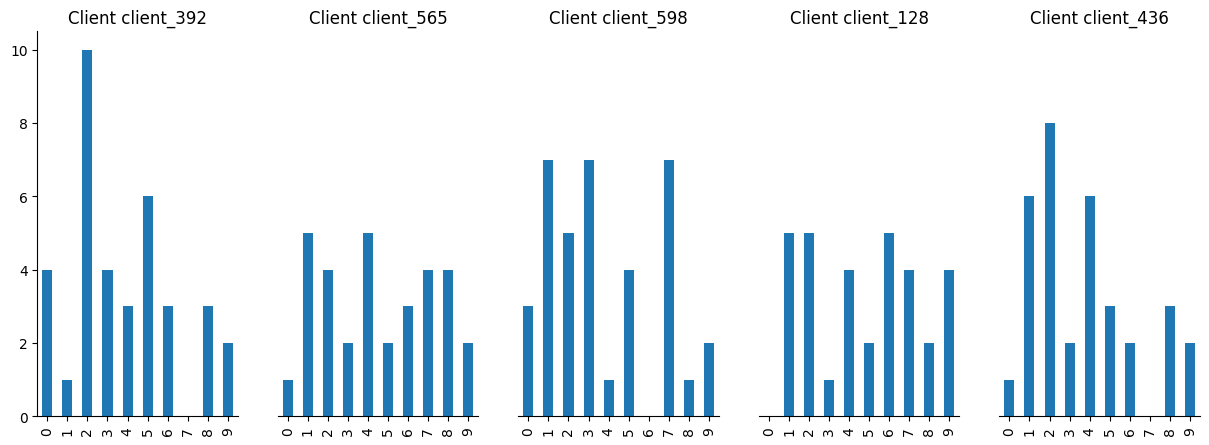
\includegraphics[width=\textwidth]{Bilder/svhn_client_label_distribution.png}
	\caption{}
	\label{fig:svhn-client-label-dist}
\end{figure}

\subsection{CIFAR100}

Die Aufgabe für den CIFAR-100 Datensatz ist wie bei den anderen eine Bildklassifizierung. Die Bilder enthalten Fotos von Dingen in der realen Welt. Zu jedem Bild gibt es zwei Klassen: einmal die grobe Klassifizierung (20 unterschiedliche Klassen) und die genaue Klassifizierung (100 Klassen), welche jeweils Unterklassen der groben Klassen bilden.

In Tensorflow Federated ist der Datensatz auf 500 Clients im Trainings- und 100 Clients im Testdatensatz aufgeteilt, von denen jeder 100 Bilder hat. Die Aufteilung der Bilder auf die Clients ist nicht zufällig, sondern es wurde eine für jeden Client eine Verteilung von den groben und genauen Klassen festgelegt. Dann wird wiederholt eine Klasse gezogen und dem Client ein zufälliges Beispiel aus dieser Klasse zugewiesen. Wenn die Beispiele einer Klasse zugewiesen sind, wird die Klasse entfernt und die Klassenverteilungen der Clients werden neu berechnet.\footnote{\url{https://www.tensorflow.org/federated/api_docs/python/tff/simulation/datasets/cifar100/load_data} (accessed 2024-06-21)} Wie heterogen die Verteilung auf den Clients ist, ist in \autoref{fig:cifar-client-label-dist} zu sehen.

Bei dem Datensatz wurde vor allem darauf geachtet, realistische Objekte alleine auf den Bildern zu haben \parencite[p.52f.]{krizhevsky:2009}.

In meinen Experimenten nutze ich die grobe Klassifizierung, um die Aufgabe einfacher zu halten.

\begin{figure}[tb]
    \centering
    \begin{subfigure}{0.4\textwidth}
		\centering        
        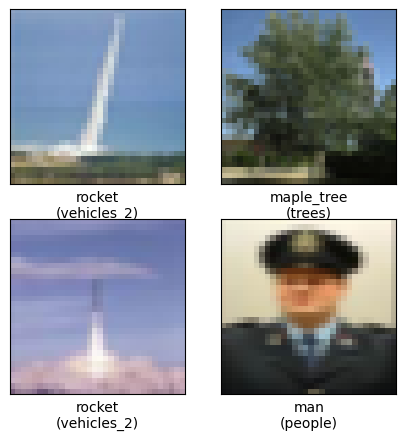
\includegraphics[width=\linewidth]{Bilder/cifar_client1.png}
        \caption{Client \texttt{238}}
    \end{subfigure}
    \hfill
    \begin{subfigure}{0.4\textwidth}
    		\centering        
        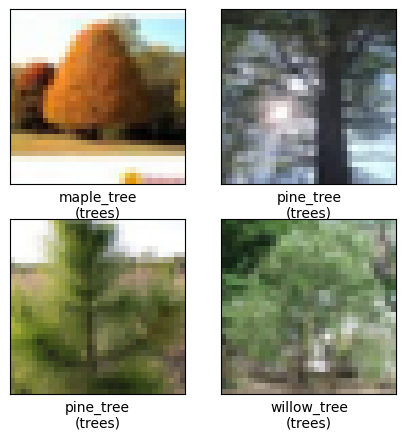
\includegraphics[width=\linewidth]{Bilder/cifar_client2.png}
        \caption{Client \texttt{423}}
    \end{subfigure}
    	\caption{Images of different clients. The images weren't partitioned randomly. The coarse label is denoted in parenthesis.}
    \label{fig:cifar-images}
\end{figure}

\begin{figure}[tb]
	\centering
	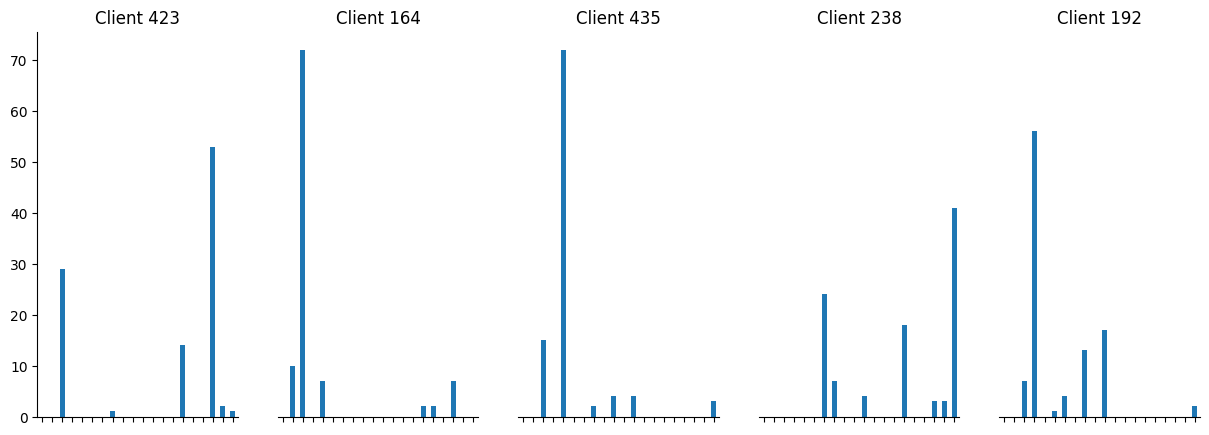
\includegraphics[width=\textwidth]{Bilder/cifar_client_label_distribution.png}
	\caption{Despite the fact that there are 2500 examples for each class in the CIFAR-100 dataset, in the tff version they are distributed very heterogeneously among the clients.}
	\label{fig:cifar-client-label-dist}
\end{figure}

\section{Models}

Die Modelle, die ich für die verschiedenen Datensätze nutze sind Convolutional Neural Networks. Um die Zeit für das Training möglichst zu minimieren, habe ich lokal mit selbst definierten, kleinen Netzen experimentiert, anstatt beispielsweise ein VGG oder ResNet zu nutzen. Ziel des Trainings war es, bereits gute Modelle und Hyperparameter zu finden und diese dann auf das Federated Learning zu übertragen. Die Ergebnisse der lokalen Modelle sind in \autoref{sec:local-training-results} beschrieben.

\section{Method}

Für meinen Algorithmus nutze ich zunächst Algorithm 2 von \textcite{boenisch:2023}. Dieser ermittelt aufgrund von individuellen Privacy Budgets die Sampling Rates und den Noise Multiplier für das Training. Da ihr Verfahren lokal ohne Federated Learning arbeitet, habe ich die nötigen Parameter folgendermaßen auf mein Federated Learning Setting übertragen:

\begin{itemize}
	\item die Anzahl der Iterationen $I$ ersetze ich durch die Anzahl der Runden in meinem Federated Learning
	\item die Anzahl der Datenpunkte ersetze ich durch die Anzahl der Clients
\end{itemize}

Der Grund für diese Ersetzungen ist, dass ich keine record-level Privacy Garantien, sondern user-level Garantien erfüllen will.

